  \documentclass[12pt,a4paper]{article}
  % Pacotes para o português.
  \usepackage[brazilian,provide=*]{babel}
  \usepackage[T1]{fontenc}
  \usepackage{times}
  \usepackage{graphicx}
  \usepackage{xcolor}
  \usepackage{indentfirst}
  \usepackage{url}
  \usepackage{array}
  \usepackage{hyperref} 
  \usepackage[top=3cm, bottom=2cm, left=3cm, right=2cm]{geometry}
  \usepackage{multirow}
  \usepackage{amssymb}
  \usepackage{amsmath}
  \usepackage{caption}
  \usepackage{setspace}
  \usepackage{breakcites}
  \usepackage{float}
  \usepackage{fancyhdr}
  \usepackage{lipsum}
  \usepackage[numbers]{natbib}
  % Tabelas com qualidade de publicação
  \usepackage{booktabs}
  \usepackage{tikz}
  \usetikzlibrary{shapes.multipart, arrows.meta, positioning, fit}
  \usepackage{enumitem}
  \setlist[itemize]{itemsep=3pt, parsep=0pt, topsep=4pt, partopsep=0pt}
  \usepackage{sectsty}
  \usepackage[compact]{titlesec}
  \newcommand{\sectionstyle}{\thispagestyle{plain}
  \sectionfont{\normalfont\large\bfseries}
  \subsectionfont{\normalfont\normalsize\bfseries}
  \subsubsectionfont{\normalfont\normalsize\bfseries}
  }
  % Comando para marcar o texto para revisão.
  \newcommand{\rev}[1]{\textcolor{red}{#1}}
  % Permite escrever aspas normais "text" em vez de ``text''
  \usepackage[autostyle]{csquotes}
  \MakeOuterQuote{"}

  \begin{document}

  % Titulo
  \titleformat{\section}
  {\normalfont\large\bfseries}
  {\thesection}{1em}{}
  
\newcommand{\p}{\rule[-0.8mm]{26mm}{3.5mm}}

\begin{document}

\begin{center}

\rule{\textwidth}{0.6pt}
\vspace{0.01cm}

{\Large\bfseries
%Aumento de dados em conjuntos de imagens histopatológicas: uma abordagem híbrida de aprendizado profundo e reconstrução volumétrica
Relatório sobre a Atividade A*
}

\rule{\textwidth}{0.6pt}

\vspace{0.5cm}

  \vspace{4cm}
  \begin{center}
  \begin{minipage}{0.45\textwidth}
      \centering
      {\large Felipe Gomes da Silva}
    \href{mailto:aluno.email@unesp.br}{felipe.gomes-silva@unesp.br}
  \end{minipage}
  \hfill
  \begin{minipage}{0.45\textwidth}
      \centering
    {\large Luis Henrique Salomão Lobato} 
  \href{mailto:aluno.email@unesp.br}{lhs.lobato@unesp.br}
\end{minipage}
\footnote{Ambos os autores contribuíram igualmente para o desenvolvimento deste trabalho.}
\end{center}
\vspace{1cm}


Instituto de Biociências, Letras e Ciências Exatas -- IBILCE \\
Universidade Estadual Paulista (UNESP) \\
São José do Rio Preto -- SP, Brasil \\

\vspace{0.1cm}


\end{center}

\newpage

\tableofcontents 

\newpage

\section{Introdução}

O quebra-cabeça de 8 peças é um problema clássico de busca em Inteligência Artificial. Consiste em um tabuleiro $3\times3$ com oito peças numeradas e um espaço vazio, no qual o objetivo é transformar uma configuração inicial em uma configuração objetivo por meio de movimentos horizontais ou verticais das peças adjacentes ao espaço vazio.
 
Embora o espaço de estados desse problema seja finito — com apenas $9! = 362.880$ configurações possíveis, das quais metade é alcançável a partir de qualquer estado inicial —, a busca cega (não informada) pode tornar-se ineficiente à medida que a profundidade da solução aumenta. Para contornar essa limitação, utiliza-se a \textbf{busca informada}, que incorpora conhecimento específico do domínio por meio de funções heurísticas.
 
Neste trabalho, implementamos o algoritmo \textbf{A*} em Python para resolver o quebra-cabeça de 8 peças, avaliando e comparando duas heurísticas admissíveis:
\begin{itemize}
    \item $h_1$: número de peças fora de lugar;
    \item $h_2$: soma das distâncias de Manhattan de cada peça em relação à sua posição objetivo.
\end{itemize}
 
O A* seleciona os nós a expandir minimizando a função $f(n) = g(n) + h(n)$, onde $g(n)$ é o custo acumulado desde o estado inicial até o nó $n$ e $h(n)$ é a estimativa heurística do custo restante até o objetivo. Quando a heurística é admissível — isto é, nunca superestima o custo real —, o A* garante encontrar a solução ótima.
 
Os experimentos foram conduzidos gerando instâncias com níveis crescentes de dificuldade (profundidade $d$), executando pelo menos 100 problemas aleatórios por nível, e registrando o número de nós gerados, o tempo de execução e o fator de ramificação efetivo $b^*$. Os resultados são discutidos nas seções seguintes.

\section{Resultados}

\noindent Como auxílio nas respostas, veja os gráficos nas Figuras~\ref{fig:bstar} e~\ref{fig:tempo}.

\begin{figure}[H]
    \centering
    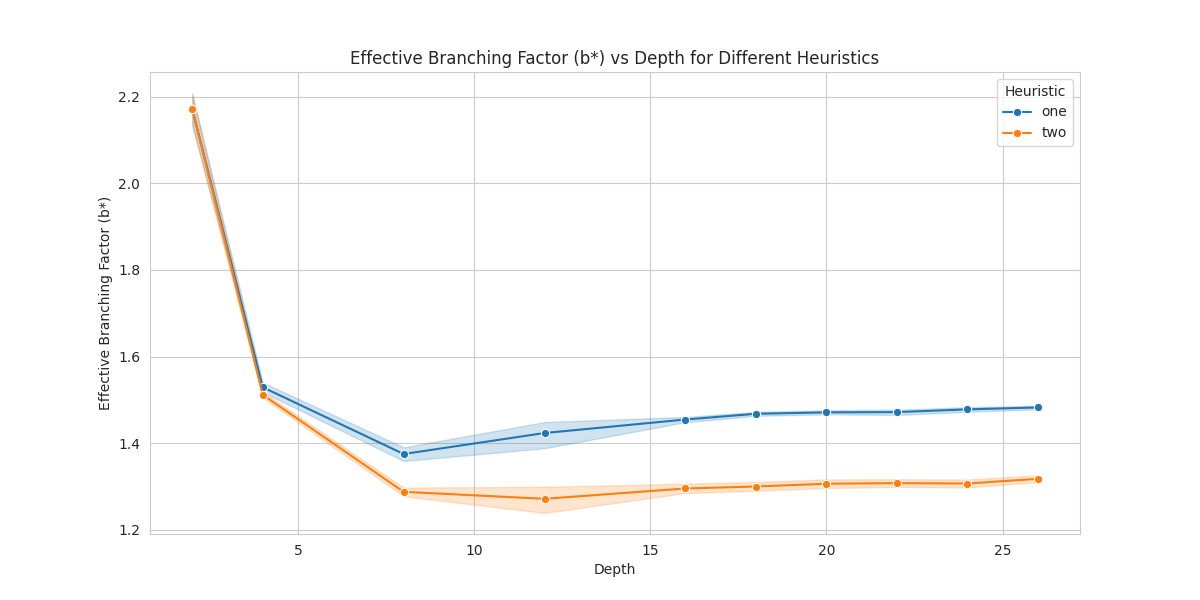
\includegraphics[width=0.85\textwidth]{../assets/b_star_vs_depth.png}
    \caption{Fator de ramificação efetivo $b^*$ em função da profundidade $d$ para as heurísticas $h_1$ e $h_2$.}
    \label{fig:bstar}
\end{figure}

\begin{figure}[H]
    \centering
    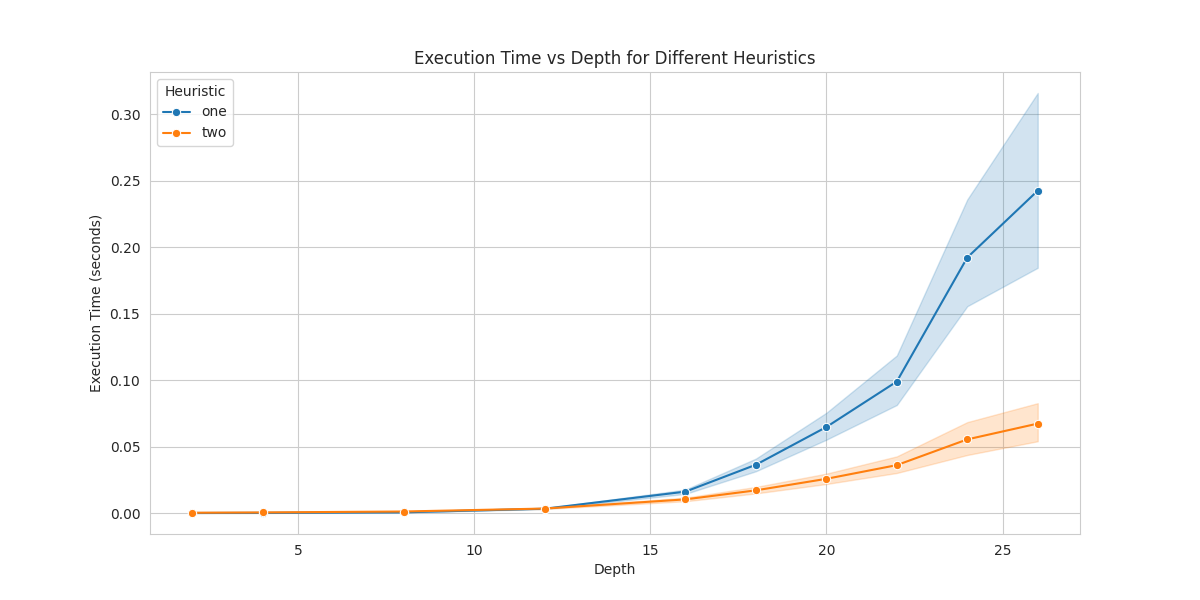
\includegraphics[width=0.85\textwidth]{../assets/execution_time_vs_depth.png}
    \caption{Tempo de execução (s) em função da profundidade $d$ para as heurísticas $h_1$ e $h_2$.}
    \label{fig:tempo}
\end{figure}

\vspace{1em}

% -------------------------------------------------------
\noindent\textbf{Questão 1.} \textit{Qual heurística apresentou o menor número de nós gerados e o menor fator de ramificação efetivo ($b^*$)?}

\vspace{0.5em}
\noindent A heurística $h_2$ (distância de Manhattan) apresentou menor fator de ramificação efetivo $b^*$ (curva laranja abaixo da azul na Figura~\ref{fig:bstar}) e menor tempo de execução em todas as profundidades, sendo claramente superior em eficiência.

\vspace{1.5em}

% -------------------------------------------------------
\noindent\textbf{Questão 2.} \textit{É correto afirmar que $h_2$ domina $h_1$? Como essa relação impacta matematicamente o número de nós expandidos pelo algoritmo A*?}

\vspace{0.5em}
\noindent Sim. $h_2$ domina $h_1$, e os gráficos confirmam isso sem contradição: como $h_2$ estima valores mais próximos do custo real, o A* expande menos nós, resultando em $b^*$ menor e tempo de execução significativamente menor. Isso ocorre pois, para qualquer estado $n$, vale $h_2(n) \geq h_1(n)$: a distância de Manhattan considera não apenas se a peça está fora de lugar, mas também o mínimo de movimentos necessários para reposicioná-la, fornecendo uma estimativa mais informada. Matematicamente, uma heurística dominante permite que A* poda mais ramos da árvore de busca, reduzindo o número total de nós $N$ gerados e, consequentemente, o $b^*$ calculado pela equação:
\[
N + 1 = 1 + b^* + (b^*)^2 + \cdots + (b^*)^d.
\]
Isso é especialmente visível em profundidades maiores, onde $h_1$ chega a ${\sim}0{,}25$\,s contra ${\sim}0{,}06$\,s de $h_2$ (Figura~\ref{fig:tempo}).

\vspace{1.5em}

% -------------------------------------------------------
\noindent\textbf{Questão 3.} \textit{Por que ambas as heurísticas são consideradas admissíveis? O que aconteceria com a otimalidade do algoritmo se a heurística superestimasse o custo real?}

\vspace{0.5em}
\noindent Ambas são admissíveis pois nunca superestimam o custo real para alcançar o objetivo:
\begin{itemize}
    \item $h_1$ conta peças fora de lugar — cada uma precisa de pelo menos 1 movimento, logo $h_1(n) \leq h^*(n)$.
    \item $h_2$ soma as distâncias de Manhattan — cada peça precisa de pelo menos esse número de movimentos para chegar à posição objetivo (sem considerar colisões), logo $h_2(n) \leq h^*(n)$.
\end{itemize}
Os valores de $b^*$ próximos de $1{,}3$–$1{,}5$ obtidos nos experimentos confirmam que o algoritmo está encontrando soluções ótimas. Se uma heurística superestimasse o custo real (heurística inadmissível), o A* poderia descartar caminhos que levam à solução ótima, pois o nó correspondente teria $f(n) = g(n) + h(n)$ artificialmente elevado, fazendo com que o algoritmo retornasse soluções subótimas.

\vspace{1.5em}

% -------------------------------------------------------
\noindent\textbf{Questão 4.} \textit{Qual é a principal limitação do A* ao lidar com problemas de maior escala (como o quebra-cabeça de 15 peças) e como o armazenamento dos nós impacta a memória?}

\vspace{0.5em}
\noindent A limitação principal do A* é o crescimento \textbf{exponencial de memória}: o algoritmo precisa manter na borda (fila de prioridade) e no conjunto de explorados todos os nós gerados, cujo número cresce como $O((b^*)^d)$. Pelo gráfico de tempo (Figura~\ref{fig:tempo}), mesmo em profundidade $d \approx 27$ o tempo já explode para $h_1$; para o quebra-cabeça de 15 peças, as soluções ótimas possuem profundidades na casa de 50 ou mais movimentos, o que exigiria armazenar bilhões de nós, tornando o A* padrão inviável em termos de memória. Uma alternativa é o algoritmo \textbf{IDA*} (Iterative Deepening A*), que combina a busca em profundidade iterativa com a heurística admissível, eliminando a necessidade de manter toda a borda em memória ao custo de reexpandir alguns nós.

\end{document}
